\section{Lecture 31}
\subsection{Lecture Notes - The Strain Tensor and Hooke's Law for Solids}
\subsubsection{The Stress Tensor}
Recall we can write the vector area element as $d\v{A} = \hat{\v{n}}dA$. What is then the stress tensor? We consider the force on a surface element $\v{F}(d\v{A})$, which we can express using the stress tensor:
\[\v{F}(d\v{A}) = \sigma d\v{A}\]
Where $\sigma$ is the stress tensor, which is a 3x3 matrix. We could alternatively write this as:
\[F_i(d\v{A}) = \sum_{j=1}^3 \sigma_{ij}dA_j\]

\subsubsection{Stress Tensor Elements}
Let
\[F_1(\text{On area dA normal to} \hat{\v{e}}_1) = \sigma_{11}dA\]
This is of course true for $\sigma_{22}$ and $\sigma_{33}$. $\sigma_{ii}$ is therefore ith component of the force $\perp$ to the i-axis. These are volumetric forces, and this tells us that the tensile and compressive forces correspond to the diagonal entries of the stress tensor. Next, consider \[F_2(\text{on area dA normal to } \hat{\v{e}}_1) = \sigma_{21}dA\]
And similarly for $\sigma_{31}$. These are clearly shearing forces, forces that act perpendicular to the plane.

\subsubsection{Symmetry of the Stress Tensor}
We said above that the stress tensor has 9 entries (3x3) but there is good news; it turns out that the tensor is actually symmetric (i.e. just 6 components to worry about!). To see this, consider the following geometry:
\begin{center}
    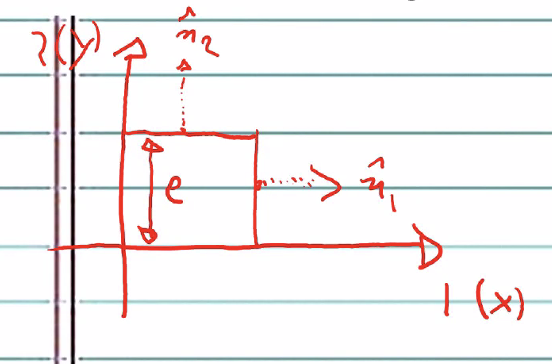
\includegraphics[scale=0.8]{Lecture-31/l31-img1.png}
\end{center}
We now apply a force in the $1$ direction, perpendicular to the $2$ direction, i.e. $F_{a} = \sigma_{12}dA$. We can also apply a force in the $2$ direction, perpendicular to the $1$ direction, which gives $F_b = \sigma_{21}dA$. It is clear to see that these forces induce a torque. WE can also apply the same forces at the opposite corner, on the opposite direction (of equal magnitude):
\begin{center}
    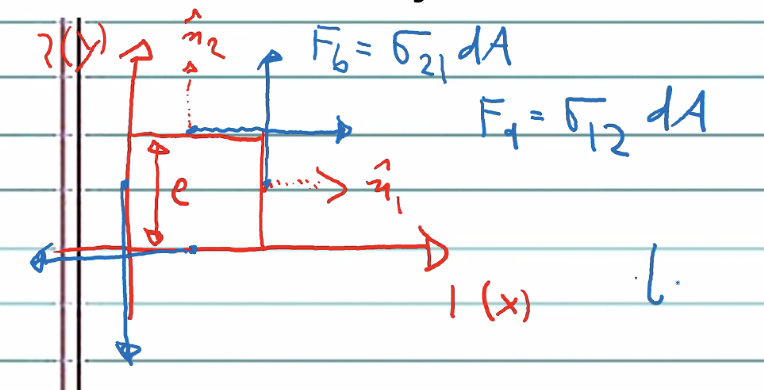
\includegraphics[scale=0.8]{Lecture-31/l31-img2.png}
\end{center}
The torque is then given by:
\[\tau = F_b l - F_q l = (\sigma_{21} - \sigma_{12})ldA = \Gamma_3\]
(this torque is in the 3-direction). Furthermore, we have that:
\[\Gamma_3 = \dod{L_3}{t}\]
We now argue that $\Gamma_3$ is zero (and hence that $\sigma_{21} = \sigma_{12}$. To see that this is the case, consider shrinking all sides of the square by a factor $\lambda$. If I change $l$ by $\lambda l$, I pick up a factor of $\lambda$, and the area picks up a factor of $\lambda^2$, for a total scaling of:
\[\Gamma_3 \mapsto \lambda_3 \Gamma_3\]
Then, what happens to the angular momentum? We pick up $\lambda^2$ from the $\v{r} \times \v{p}$, and then integrating over the plane, we have that we pick up a $\lambda^2$, so it follows that:
\[\lambda^3\Gamma_3 = \lambda^4\dod{L_3}{t}\]
But this is ture for all $\lambda$, so it follows that $\Gamma_3$ must be zero, and hence $\sigma_{21} = \sigma_{12}$. An identical argument shows that $\sigma_{ij} = \sigma{ji}$ in general.

\subsubsection{Displacements}
We now have a measure of force on the system, but we also need a measure of deformation. In general, we can write down a vector $\v{r}$ from the origin to any position in the original configuration, and we change this $\v{r}$ to a new vector $\v{r} + \v{u}(\v{r})$ where $\v{u}$ is the displacement from the reference to the current position. 
\begin{center}
    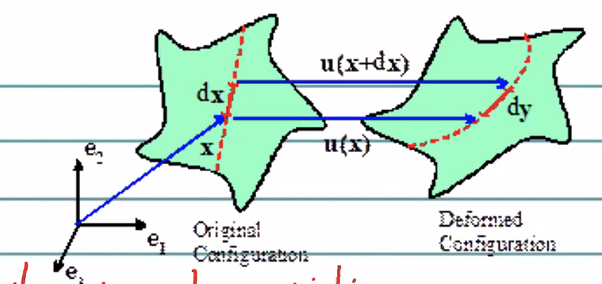
\includegraphics[scale=0.8]{Lecture-31/l31-img3.png}
\end{center}
This displacement vector in general depends on the position, not all points in the object will move the same amount. One might ask why do we want $\v{r} + \v{u}(\v{r})$ and not just $\v{u}$ by itself; consider that $\v{u}$ itself would change during a constant translation ($\v{u}(\v{r}) = \v{u}_0$) of the entire object, and hence is not a good measure of the strain. We need to look at \textbf{distortions}. A general way to write down/pick up these distortions:
\[du_i = \sum_{j}\dpd{u_i}{r_j}dr_j\]
Or we can write this vectorially:
\[d\v{u} = \DD d\v{r}\]
Where:
\[\DD = \m{\dpd{u_1}{r_1} & \dpd{u_1}{r_2} & \dpd{u_1}{r_3} \\ \dpd{u_2}{r_1} & \dpd{u_2}{r_2} & \dpd{u_2}{r_3} \\
\dpd{u_3}{r_1} & \dpd{u_3}{r_2} & \dpd{u_3}{r_3}}\]
And this matrix contains the rate of change of the displacement. This is nice, as evidently this is now insensitive to any constant translations. The gradient of the constant translation will be zero, which is what we want as we should not have to pay any energy just by moving our rigid body back and forth.

\subsubsection{The Strain Tensor}
But there is another wrinkle to consider; rotating the body should also not change the energy of the body/the energy should not depend on the orientation. What do we then do about rotations?
COnsider that for a small rotation:
\[\bm{\theta} = \theta\v{u}\]
About an axis $\v{u}$. To see this, 
\[\v{v} = \bm{\omega} \times \v{r}\]
So we can use this to write:
\[\v{u}(\v{r}) = \v{v}dt = \bm{\omega} dt \times \v{r} = \bm{\theta} \times \v{r}\]
Then we have that the displacement gradient has the form:
\[\DD = \m{0 & \theta_3 & -\theta_3 \\ -\theta_3 & 0 & \theta_1 \\ \theta_2 & -\theta_1 & 0}\]
Which we can see is an antisymmetric matrix. The antisymmetry means that:
\[\DD^T = -\DD\]
We need to get rid of this; we dont want a measure that picks up these rotations. We can construct this by remembering that any matrix can be decomposed into a symmetric and antisymmetric part. So, we write:
\[\DD = \frac{1}{2}(\DD - \DD^T) + \frac{1}{2}(\DD + \DD^T)\]
Where the first term is by construction anti-symmetric, and the second term is by construction symmetric. Hence, we will just keep the second term, and use this as the measure of strain. The first term corresponds to the vorticity/curl part, but here we only want to keep the symmetric part. Hence, we can define the small-strain tensor as:
\[\e = \frac{1}{2}\left(\DD + \DD^T\right)\]
Which we can see is symmetric by construction;
\[\e_{ij} = \frac{1}{2}\left(\dpd{u_i}{r_j} + \dpd{u_j}{r_i}\right)\]

\subsubsection{Example: Thin/thick plate in xy plane}
Consider a thin plate subject to in plane (xy) tensile, compressive, or shear forces. Are $\sigma_{zz}$ and $\e_{zz}$ zero? nonzero?
\begin{center}
    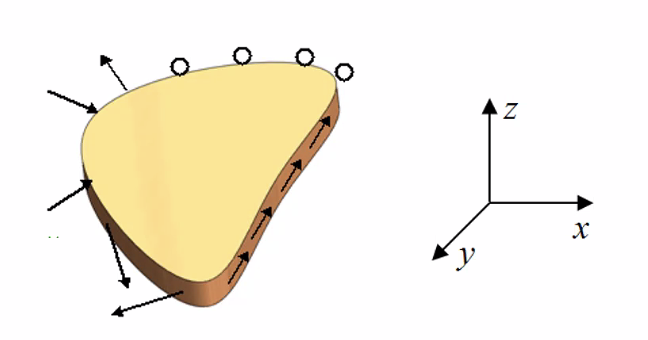
\includegraphics[scale=0.8]{Lecture-31/l31-img4.png}
\end{center}
\begin{s}
$\sigma_{zz} = 0$ and $\e_{zz} \neq 0$. For the first point, we can recognize that pulling on the plate in the xy plane induces no stress on the plane in the z direction. For the second point, we consider a sheet of rubber which changes in thickness as we pull it.
\end{s}
What if we ask the same question, but this time the plate is thick?
\begin{s}
If we compare the thick to the thing plate, any length change from the contraction effect would be very very small as the rod is tall. Hence, if we elongate it a little bit, then to first order, there is no strain. But, there can be a stress, as the system would like to contract.
\end{s}

The first case (thin plate) corresponds to a plane stress condition. There is no stress in the z-axis, but if we pull, we get an appreciable change in the thickness of the plate and hence a nonzreo strain. On the other hand, we have the plane strain condition, where there is no strain in the z axis (rod is so tall such that the strain in the z-direction is negligeble/the rod does not change thickness when we pull) but we could still have a stress in the z-axis.

\subsubsection{Hooke's Law for Isotropic and Homogenous Solids}
Consider a decomposition of strain tensor. Consider the quantity of average dilation:
\[e = \frac{1}{3}(\e_{11} + \e_{22} + \e_{33}) = \frac{1}{3}\Tr(\e)\]
Which is a measure of how much the system is compressed/pulled. The last equality we just write the expression as the trace of the strain tensor. Then, decomposing we have:
\[\e = e\II + \e^{dev} = \text{Vol}(\e) + \text{Dev}(\e)\]
Where the first term is the spherical term (the term that couples to the volume changes) and the second term is the deviatoric part (everything else, e.g. shear). Then, Hooke's Law says that:
\[\sigma = f(\e)\]
Where $f$ is a linear function. Then, we write (Without proof) that in the linear case, we can use this decomposition to obtain:
\[\sigma = 3B\text{Vol}(\e) + 2G\text{Dev}(\e)\]
Where $B$, $G$ are the bulk and shear moduli. We can alternatively write this as:
\[\sigma = 2\mu\e + \lambda \Tr(\e) \II\]
Where $\mu = G$ and $\lambda = B - \frac{2}{3}\mu$. What is important to realize is that this is true for an isotropic and homoegnous solid, in which case only two elastic moduli are sufficient to characterize this response (we only need to know the bulk and shear moduli). Of course in something like an anisotropic metal, this would be more complicated.